% title of the dissertation
\def\distitle{Interference and Scattering in Surface Plasmon Resonance}
\usepackage{mathtools}
\usepackage{t1enc}
\usepackage[T1]{fontenc}
\usepackage[utf8]{inputenc}
\usepackage{ulem}
\usepackage{import}
\usepackage{amsmath}
\usepackage{amssymb}
\usepackage{paralist}
\usepackage{booktabs}
\usepackage[version=3]{mhchem}
\usepackage{wrapfig}
\usepackage{pifont}
\usepackage{mathrsfs}
\usepackage{xcolor}
\usepackage{color}
\usepackage{enumitem}
\usepackage{datetime}
\usepackage{fullpage}
\usepackage{attachfile}
\usepackage{textpos}
\usepackage{rotating}
\usepackage{ifthen}
\usepackage[parfill]{parskip}
%\usepackage{minted}
\usepackage[inline]{showlabels}
\usepackage{subcaption}

\usepackage{hyperref}
\hypersetup{
 colorlinks=false,
 hidelinks=true,
}

\usepackage{pgfplots}
\usepackage{pgfplotstable}
\pgfplotsset{compat=newest}
\usepgfplotslibrary{units}
\usepgfplotslibrary{external}
\pgfplotsset{filter discard warning=false}

\usepackage[siunitx]{circuitikz}
\usepackage{pgf,tikz}
\usetikzlibrary{calc}
\usetikzlibrary{patterns,decorations.pathmorphing,decorations.markings,positioning}
\usetikzlibrary{pgfplots.units} 
\usetikzlibrary{pgfplots.external} 
\usetikzlibrary{pgfplots.groupplots}
\usetikzlibrary{arrows}
\usetikzlibrary{plotmarks}

\tikzexternalize[prefix=external/]% externalize

% my pretty colors
\import{colors/}{colors}

% siunitx
\usepackage{siunitx}
\sisetup{ 
binary-units,
% load-configurations=abbreviations
% round-mode = places,
}%
\DeclareSIUnit\molar{\mole\per\cubic\deci\metre}
\DeclareSIUnit\Molar{\textsc{m}}
\DeclareSIUnit\torr{torr}

% prettify chapter/section format
\usepackage{titlesec}
\newcommand{\hsp}{\hspace{20pt}}
\titleformat{\chapter}[hang]{\Huge\bfseries}{\thechapter\hsp\textcolor{gray}{|}\hsp}{0pt}{\Huge\bfseries}
% New definition of square root:
% it renames \sqrt as \oldsqrt
% This definition puts a little vertical guy at the end so it's more
% obvious where the square root actually ends.
\let\oldsqrt\sqrt
% it defines the new \sqrt in terms of the old one
\def\sqrt{\mathpalette\DHLhksqrt}
\def\DHLhksqrt#1#2{%
\setbox0=\hbox{$#1\oldsqrt{#2\,}$}\dimen0=\ht0
\advance\dimen0-0.2\ht0
\setbox2=\hbox{\vrule height\ht0 depth -\dimen0}%
{\box0\lower0.4pt\box2}}

% integrals with infinity bounds
\newcommand{\intinfty}{\int_{-\infty}^{\infty}}

% consistent formatting of object labels
\newcommand{\Figure}[1]{Figure~\ref{#1}}
\newcommand{\Equation}[1]{Equation~\ref{#1}}
\newcommand{\Table}[1]{Table~\ref{#1}}
\newcommand{\Section}[1]{Section~\ref{#1}}
\newcommand{\Chapter}[1]{Chapter~\ref{#1}}
\newcommand{\Part}[1]{Part~\ref{#1}}
\newcommand{\Appendix}[1]{Appendix~\ref{#1}}

% I want all of the document numbering to always show the full path, fuck
% with this later
%\renewcommand\thesection{\Roman{part}.\Alph{chapter}.\arabic{section}}
%\renewcommand\thesubsection{\arabic{section}.\arabic{subsection}}
%\renewcommand\thesubsubsection{\arabic{subsection}.\arabic{subsubsection}}

%\renewcommand\thefigure{S\arabic{figure}}
%\renewcommand\thesection{\Roman{part}.\arabic{chapter}.\arabic{section}}
%\renewcommand\thetable{S\arabic{table}}

% names have a particular formatting
\newcommand{\name}[1]{\textsc{#1}}

% missing mathematical operators
\DeclareMathOperator{\sinc}{sinc}
\DeclareMathOperator{\sech}{sech}
\DeclareMathOperator{\sgn}{sgn}
\DeclareMathOperator{\erf}{erf}
\DeclareMathOperator{\inverf}{inverf}
\DeclareMathOperator{\arcsinh}{arcsinh}
\DeclareMathOperator{\arccosh}{arccosh}
\DeclareMathOperator{\arctanh}{arctanh}
%\DeclareMathOperator{\Re}{Re}
%\DeclareMathOperator{\Im}{Im}

% use roman type for natural base e and sqrt(-1)
\newcommand{\me}{{\mathrm{e}}}
\newcommand{\mi}{{\mathrm{i}}}

% roman type for the derivative, plus a space
\newcommand{\md}{\,\mathrm{d}}

% fourier transform and the reverse
\newcommand{\ff}[1]{{\mathscr{F}^{+}\bigl(#1\bigr)}}
\newcommand{\fr}[1]{{\mathscr{F}^{-}\bigl(#1\bigr)}}

% hilbert transform and the reverse
\newcommand{\hf}[1]{{\mathscr{H}^{+}\bigl(#1\bigr)}}
\newcommand{\hr}[1]{{\mathscr{H}^{-}\bigl(#1\bigr)}}

% QCM related frequency and bandwidth shifts
\newcommand{\df}{\Delta\!f}
\newcommand{\dg}{\Delta\Gamma}
\newcommand{\xil}{\xi_\mathrm{L}}
\newcommand{\kl}{k_\mathrm{L}}
\newcommand{\ml}{m_\mathrm{L}}
\newcommand{\kq}{k_\mathrm{q}}
\newcommand{\mq}{m_\mathrm{q}}
\newcommand{\omegaq}{\omega_\mathrm{q}}
\newcommand{\thetasp}{\theta_\mathrm{sp}}

\newcommand{\ersatzfigure}{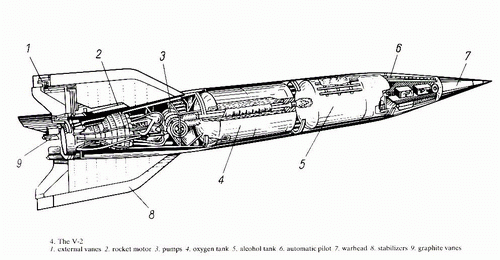
\includegraphics[width=10cm,keepaspectratio]{includes/ersatz}}
